\chapter{Concepts}
Pour parvenir à créer une machine capable de trier des billes de roulement à bille, il nous a fallu résoudre deux problèmes: l'acheminement des billes, et leur tri.

%\section{Répartition du projet}

Vu que nous étions un groupe de quatre étudiants, nous avons décidé de répartir la machine en quatre parties. Les deux problèmes principaux susmentionnés ont été les deux divisés en deux. Ensuite, chacun de nous s'est occupé de concevoir le/les mécanisme/s nécessaire/s pour que la machine dans son ensemble puisse satisfaire les conditions imposées par le cahier des charges. Notre division fut la suivante:
\begin{itemize}
    \item Réservoir pour les billes mixtes
    \item Acheminement
    \item Séparation \& tri
    \item Réservoirs pour les billes triées
\end{itemize}

\section{Réservoir pour billes mixtes}

\subsection{Concepts imaginés}
Nous avons dans un premier temps imaginé un réservoir rectangulaire, en forme de parallélépipède creux. Mais l’usinage d’une telle pièce exige le forage d’un cube de métal, ce qui entraîne un important gaspillage.

Ensuite, l’idée d’un cylindre creux associé à un fond sphérique est apparue comme étant la plus économe et la plus rapide à assembler. En effet, le cylindre peut être un simple tuyau coupé à la bonne longueur et usiné sur un seul côté pour permettre la sortie du réservoir. Le fond incliné consiste en une plaque sphérique usinée pour obtenir l'inclinaison nécessaire à l'évacuation des billes. De plus, les deux pièces peuvent facilement être assemblées grâce à 2 vis.

\begin{figure}
    \centering
    \includegraphics[width=\textwidth]{Graphics/Reservoir_initial/RESERVOIR_CYLINDRIQUE.pdf}
    \caption{Réservoir cylindrique}
    %\label{fig:B4}
\end{figure}

Après, nous avons conçu un réservoir en deux pièces usinées, pour répondre aux exigences de formes à l'entrée du distributeur. En effet, une rampe d'accès rectangulaire était plus pratique et plus simple que celle du réservoir cylindrique. De plus, seulement deux vis sont nécessaires pour assembler les pièces du réservoir. 
\begin{figure}
    \centering
    \includegraphics[width=0.5\textwidth]{Graphics/Reservoir_initial/RESERVOIR_CUBE.pdf}
    \caption{Réservoir rectangulaire}
    %\label{fig:B4}
\end{figure}

Finalement, nous avons décidé d'incorporer le réservoir au reste de la machine, pour gagner en simplicité lors de l'assemblage et pour diminuer le nombre de pièces. Ainsi, les parois latérales de la machine se prolongent pour former le réservoir initial dans lequel les billes sont versées avant leur tri. Une seule plaque supplémentaire est nécessaire pour former le fond de ce réservoir, légèrement inclinée pour assurer la descente des billes vers le distributeur. Cela simplifie l'assemblage.  Le dernier quart restera découvert, pour ne pas augmenter les frottements à l'entrée du distributeur. L'ensemble est assemblé simplement grâce à quatre goupilles. 

\section{Acheminement}
Ce mécanisme devait satisfaire plusieurs contraintes et demandes à la fois. Il était prescrit que notre machine s'opère à une main et que le tri des billes soit déclenché par l'utilisateur et ne se déclenche pas soi-même. De plus, tout coincement devait être prévenu.

Les options élaborées en groupe étaient alors les suivantes:\\
Pour l'entraînement des billes:

\subsection{Convoyeur à vis}
Notre première idée fut une convoyeur à vis qui transporte les billes vers les rails. Les billes sortent alors du réservoir mixte et roulent vers le convoyeur à vis. La rotation provenant de la manivelle les entraîne ensuite vers les rails.

\begin{figure}
    \centering
    \includegraphics[width=\textwidth]{Graphics/Images_concepts_Leon/795-Screw_conveyor.png}
    \caption{Convoyeur à vis}
    %\label{fig:B4}
\end{figure}

Mais après tout cette idée fut impraticable à cause de plusieurs raisons. Premièrement, le coût était sûrement plus élevé que celui des autres alternatives, et deuxièmement, nous ne trouvions pas de solution satisfaisante pour empêcher de manière certaine le coincement des billes.

\subsection{Cylindre avec des trous}
La deuxième option qu'on a élaboré était un long cylindre avec de petits trous usinés à sa surface. Comme avec le convoyeur à vis, les billes roulent hors du réservoir mixte et tombent dans les trous du cylindre tournant. Comme pour la première idée, nous prévoyions une manivelle pour l'opération du mécanisme.

\begin{figure}
    \centering
    \includegraphics[width=\textwidth]{Graphics/Roue/DRAWING_PROTOTYP_CYLINDRE.pdf}
    \caption{Cylindre avec trous}
    %\label{fig:B5}
\end{figure}

Cette option a finalement été abandonnée, car la fabrication aurait coûté plus cher que celle de la troisième option (cf. en bas). Nous aurions dû faire des alésages très précis au lieu de juste fraiser des roues dentées.

\subsection{Distributeur avec cylindres décalés}
Notre troisième idée était de simplement monter des cylindres sur une barre et de décaler deux roues voisines d'une dent.

\begin{figure}
    \centering
    \includegraphics[width=\textwidth]{Graphics/Roue/DRAWING_ROUES_DENTEES_DECALES.pdf}
    \caption{Cylindres perforés décalés}
    %\label{fig:B6}
\end{figure}

Les billes provenant du réservoir mixte roulent alors doucement (grâce à la pente modérée)  vers les cylindres perforés. Elles tombent ensuite entre les trous et sont entraînées vers les rails par la rotation des roues, actionnées par la manivelle.

\begin{figure}
    \centering
    \includegraphics[width=\textwidth]{Graphics/Roue/DRAWING_COUVERCLE_COMPLET.pdf}
    \caption{Roues dentées décalés (mécanisme complet)}
    %\label{fig:B7}
\end{figure}

Pour le déblocage: %altérer
\subsection{Un pivot positionné à la sortie du réservoir pour empêcher l'empilement des billes} 
Notre première option pour le déblocage fût un pivot positionné à la sortie du réservoir mixte. Ce pivot aurait été connecté à l'axe de rotation de l'acheminement par une chaîne ou une autre connexion permettant la transformation de la rotation en "pivotement". Ainsi, tout empilement pouvant créer un coincement des billes dans le réservoir aurait été empêché par l'utilisation de la manivelle.

\begin{figure}
    \centering
    \includegraphics[width=\textwidth]{Graphics/Roue/DRAWING_PIVOT.pdf}
    \caption{Pivot débloquant}
    %\label{fig:B8}
\end{figure}

\subsection{Couvercle pour la roue dentée}
Comme mécanisme de déblocage supplémentaire, nous prévoyions un couvercle pour le mécanisme d'acheminement. Avec des dents/trous d'une profondeur de 5 mm, même les billes de diamètre 7 peuvent passer sous un couvercle à distance 2,5 mm du mécanisme d'acheminement. Par contre, dès qu'il y aura deux billes dans un trou, même pour le pire des cas (deux billes de la taille la plus petite, soit 5 mm), la deuxième bille heurtera le couvercle en dessous ou exactement à la hauteur de son centre de masse. Ainsi, ce système prévient tout coincement à l'entrée des cylindres perforés et assure le passage d'une seule bille par trou.

\begin{figure}
    \centering
    \includegraphics[width=\textwidth]{Graphics/Roue/DRAWING_COUVERCLE.pdf}
    \caption{Couvercle}
    %\label{fig:B9}
\end{figure}

\begin{figure}
    \centering
    \includegraphics[width=\textwidth]{Graphics/Roue/DRAWING_COUVERCLE_DEMI_COMPLET.pdf}
    \caption{Couvercle avec fixations}
    %\label{fig:B10}
\end{figure}

\begin{figure}
    \centering
    \includegraphics[width=\textwidth]{Graphics/Roue/DRAWING_COUVERCLE_COMPLET.pdf}
    \caption{Couvercle avec mécanisme complet}
    %\label{fig:B11}
\end{figure}

\section{Séparation \& tri (rails)}

\subsection{Séparation}
Après que les billes ont été acheminées hors du réservoir, elles doivent être séparées de manière successive pour ne pas bloquer le mécanisme de tri qui suit. Comme plusieurs billes sont triées au même temps, une méthode efficace de séparation devrait nécessaire. 

\subsubsection{Coins}
La première idée que nous avons trouvé, était d'ordonner les billes en utilisant des coins sur un plan incliné. Cette méthode débouchait cependant sur plusieurs problèmes: la pièce est devenue très compliquée à fabriquer, à cause de l'usinage particulier des parties surélevées en forme d'ogive. De plus, le risque de coincement des billes ne pouvait pas être éliminé avec certitude.

\begin{figure}
    \centering
    \includegraphics[width=\textwidth]{Graphics/Rails/COINS.pdf}
    \caption{Séparation par coins}
    %\label{fig:S_Coins}
\end{figure}

\subsubsection{Rainures}
Après avoir abandonné l'idée des coins, nous avons cherché une autre solution pour guider les billes qui arrivent du convoyeur à vis sur les rails. Notre deuxième option était de séparer les billes, non pas grâce à d'autres pièces, mais par leur propre poids. Cette idée consistait en une plaque avec des rainures de forme arrondie ou linéaire. Comme les billes de deux roues du convoyeur arrivent sur un seul rail, il s'agit de la manière la plus efficace et simple pour guider les billes sur le mécanisme de tri. Pour garantir que tous les billes arrivent à la même position relatif aux rails, nous avons décidé d'usiner les rainures pas en forme arrondie, mais linéaire, en forme "V".

Nous sommes conscients que cette décision d'usiner les rainures directement dans une plaque et pas les assembler à partir des pièces plus simples, rend cette partie de la machine plus complexe à usiner, mais nous sommes arrivés à la conclusion que cette décision était nécessaire pour assurer le positionnement précis et le tri exact des billes.

%Ces deux options n'étaient pourtant pas optimales non plus, car il fallait fraiser les cercles ou les formes en "V" dans une plaque, un défaut qui augmentera beaucoup le coût de cette pièce.

\begin{figure}
    \centering
    \includegraphics[width=\textwidth]{Graphics/Rails/SEPARATEUR_V.pdf}
    \caption{Séparation par rainures en forme "V"}
    %\label{fig:S_Rainures}
\end{figure}

\subsection{Tri}
À ce point vient la partie principale de tout l'ensemble, le tri des billes en dépendance de leur diamètre.

\subsubsection{Ecartement graduel}
Notre première idée pour trier des billes, était d'utiliser des rails quasi-parallèles qui s'écartaient de manière graduelle. Nous avons rejeté ce concept assez vite, le raisonnement pour cette décision se trouve sur %ref Justification
Le problème principal de cette méthode est que les billes perdent beaucoup de leur vélocité en avançant sur les rails, ce qui mène à des bouchons et finalement au blocage du mécanisme.

\subsubsection{Ecartement séquentiel}
Pour résoudre les faiblesses de l'écartement graduel, nous l'avons adapté et sommes arrivés à un écartement séquentiel. L'avantage de cette technique est que les billes ne ralentissent pas dans leurs rails, mais roulent avec une vitesse constante, jusqu'au point où se trouve le saut d'un diamètre au prochain et elles tombent dans le réservoir correspondant au-dessous.

\begin{figure}
    \centering
    \includegraphics[width=\textwidth]{Graphics/Rails/ECARTEMENTS.pdf}
    \caption{Comparaison d'un écartement graduel (a) et d'un écartement séquentiel (b)}
    %\label{fig:Ecartements}
\end{figure}

\subsubsection{Plaque inclinée et barres}
Une idée alternative aux solutions avec les rails était de monter des barres au-dessus d'une plaque inclinée, de manière à ce que les billes avec un diamètre donné seront transportées à coté de la plaque et les billes plus petites passent au-dessous de la barre jusqu'à la prochaine. Cette idée est développée en plus de détail sur la figure %ref fig

% image

%\subsubsection{Ecartement séquentiel avec rainures}
%L'idée finale, qui a été retenue dans le projet, est celle des rails avec un écartement séquentiel en combinaison avec les rainures en forme "V", le tout en une seule pièce. Ainsi, les parties de séparation des billes et de leur tri sont combinées, et la complexité de l'ensemble est réduite au maximum.

\section{Réservoir pour les billes triées}
Les exigences pour le réservoir des billes triées sont clairs: Il nous fallait trois containers placés de sorte que toutes les billes de même diamètre tombent dans le réservoir prévu pour leur taille.

\subsection{Premier brouillon}
La construction des rails nous a donné un espace limité où les billes d'une taille tombent. Cela veut dire qu'il y a trois rectangles l'un juste à côte de l'autre. Pour simplifier la construction nous les avons choisi de la même taille, indépendant de la taille des billes. Le premier brouillon était donc un réservoir avec un fond incliné pour que les billes s'accumulent tous du même côté.

\begin{figure}
    \centering
    \includegraphics[width=\textwidth]{Graphics/Reservoir_final/PREMIER_BROUILLON.pdf}
    \caption{Premier brouillon}
    %\label{fig:B1}
\end{figure}

Les billes devaient ainsi être enlevées à la main du réservoir, ce qui peut poser des problèmes à cause de la petite taille. Nous avons alors décidé de faire des containers qui peuvent être enlevés pour récupérer les billes. 

\subsection{Deuxième brouillon}
La forme choisie pour les containers était un cube. Il nous fallait alors une rampe, afin de canaliser les billes dans les cubes. Afin d'utiliser le place de la manière la plus efficace possible, nous avons inversé l'orientation de la rampe au milieu. Ainsi, les containers ne se trouvent pas tous sur une ligne, ce qui rend la machine plus compacte. 

\begin{figure}
    \centering
    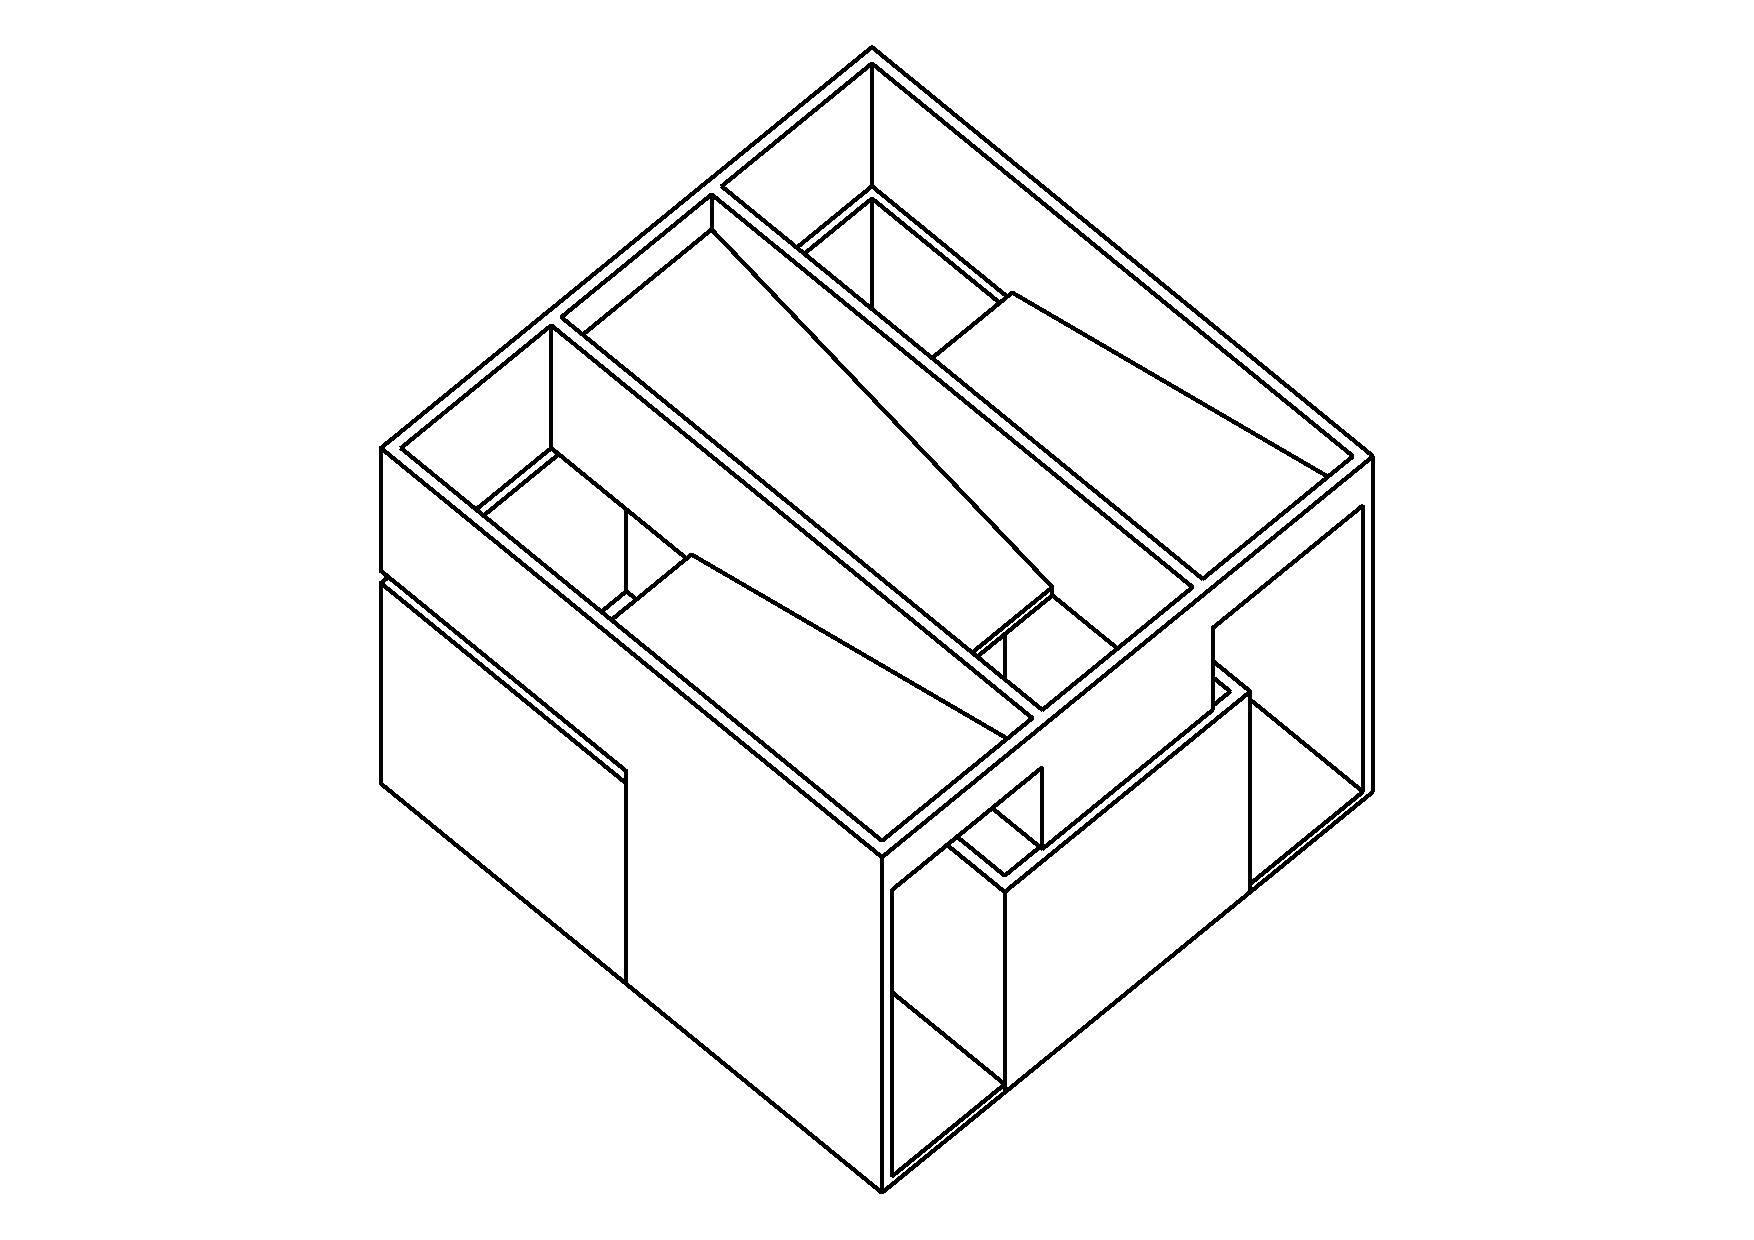
\includegraphics[width=\textwidth]{Graphics/Reservoir_final/DEUXIEME_BROUILLON.pdf}
    \caption{Deuxième brouillon}
    %\label{fig:B2}
\end{figure}

\subsection{Troisième brouillon}
Vu que l'assemblage avec des vis de plus de 4 mm n'est pas possible pour certaines éléments du deuxième brouillon (i.e. les cubes) et que la fabrication par fraisage à partir d'un seul bloc est bien trop coûteux et inefficace, nous avons remanié le brouillon en respectant ces aspects. La forme allongée des containers nous a permis de supprimer les rampes au-dessous du réservoir et donc de diminuer le nombre d'éléments.

\begin{figure}
    \centering
    \includegraphics[width=\textwidth]{Graphics/Reservoir_final/TROISIEME_BROUILLON.pdf}
    \caption{Troisième brouillon}
    %\label{fig:B3}
\end{figure}

%\section{Acheminement}
%Pour l'acheminement des billes, nous avons tout d'abord imaginé un réservoir au fond incliné contenant les billes, et débouchant sur une série de roues dentées qui permettent de réguler le flux de billes.

%Ensuite, nous avons dû imaginé un mécanisme permettant d'acheminer les billes vers la zone de tri de manière régulée, tout en évitant absolument le coincement. Ainsi, l'idée de routes dentées dimensionnées pour contenir exactement une bille dans chaque compartiment s'est imposée comme étant la meilleure. En effet, une série de roues dentées décalées d'une dent (...) permet de prélever un nombre précis de billes en vue du tri.
%Les routes dentées sont actionnées grâce à une manivelle qui transmet le mouvement de rotation grâce à un arbre.

%\section{Tri}
%Pour le tri des billes, nous avons développé un système de rails parallèles, s'écartant par pallier. Cela permet de récolter les petites billes d'abord, les moyennes ensuite et finalement les plus grosses. L'écartement par pallier permet aussi d'éviter le coincement. En effet, nous avions tout d'abord pensé à un écartement progressif des rails, mais les billes ralentissent alors fortement avant de tomber, ce qui peut provoquer l'arrêt des billes suivantes. En effet, plus le diamètre de la bille se rapproche de la distance entre les rails, plus la bille descend, et son axe de rotation se rapproche de son axe de symétrie horizontal. Il en résulte une augmentation de la vitesse de rotation de la bille, et une diminution de sa vitesse horizontale. Ainsi, la bille qui suit risque de frotter contre celle qui ralentit, et la force de frottement entre les deux, amplifiée par l'augmentation de la vitesse angulaire de la première bille, risque de stopper les billes sur le rails, bloquant alors le mécanisme.